\section{Variazione Totale}
Tramite un algoritmo possiamo recuperare immagini sfocate basandoci sulla Variazione totale partendo da una Blurring Point-Spread function di un'immagine. 

La variazione totale è definita dalla seguente formula:                                                                                

\[TV(u) = \sum_i^n{\sum_j^m{\sqrt{||\nabla u(i, j)||_2^2 + \epsilon^2}}}\]

Per calcolare il gradiente dell'immagine $\nabla u$ usiamo la funzione \code{np.gradient} che approssima la derivata per ogni pixel calcolando la differenza tra pixel adiacenti. 

I risultati sono due immagini della stessa dimensione dell'immagine in input, una che rappresenta il valore della derivata orizzontale dx e l'altra della derivata verticale dy. Il gradiente dell'immagine nel punto $(i, j)$ è quindi un vettore di due componenti, uno orizzontale contenuto in dx e uno verticale in dy.
\[x^* = \arg\min_x \frac{1}{2} ||Ax - b||_2^2 + \lambda TV(u)\] 
il cui gradiente $\nabla f$ è dato da: 
\[\nabla f(x) = (A^TAx - A^Tb)  + \lambda \nabla TV(x)\]

\subsection{Variazione totale dell'immagine fotografica:}
\begin{figure}[H]
    \centering
    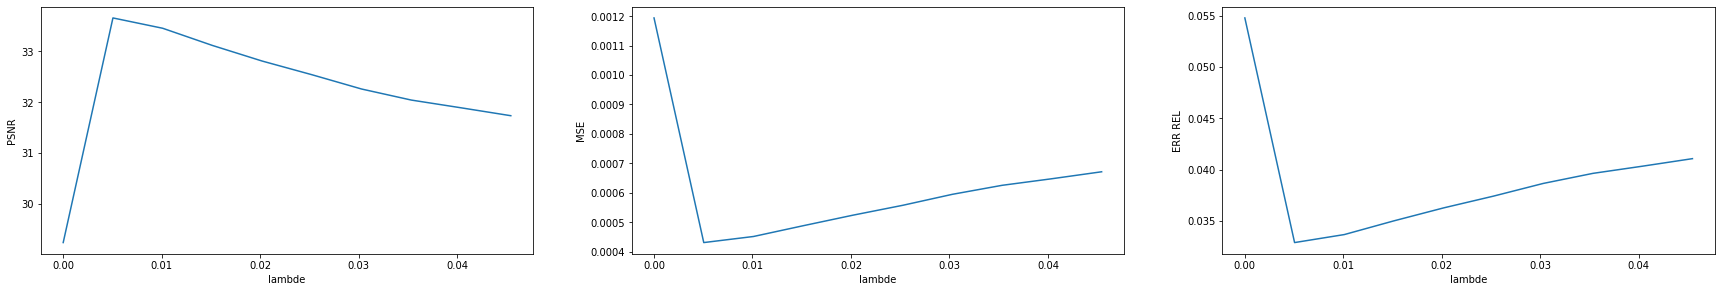
\includegraphics[width=\textwidth]{imgRel/graficoPugile.png}
    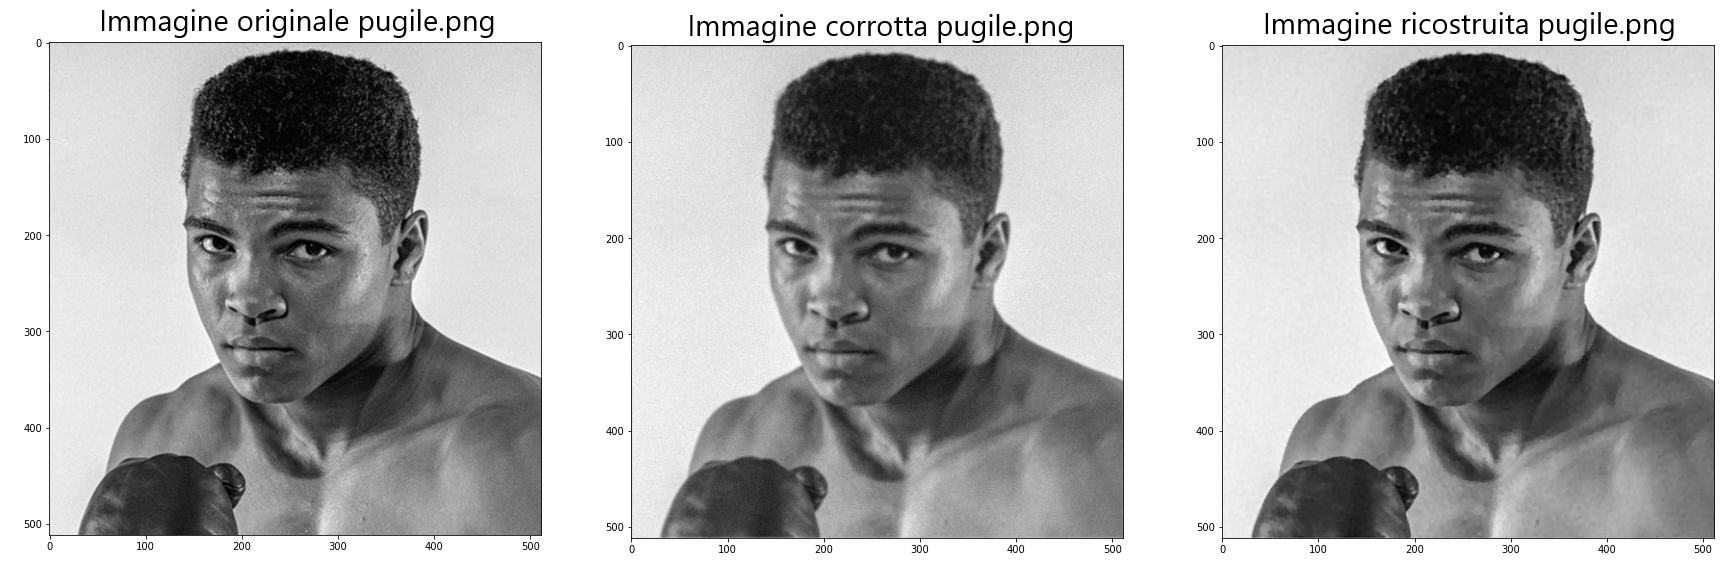
\includegraphics[width=\textwidth]{imgRicostruzione/ricostruzionePugile_TOTVAR_maxPSNR33.70.png}
    \caption{Immagine Originale, Immagine Corrotta, Immagine Ricostruita e i relativi grafici di variazione PSNR, MSE ed Errore Relativo (da sinistra a destra)}
\end{figure}

\subsection{Variazione totale dell'immagine con testo:}
\begin{figure}[H]
    \centering
    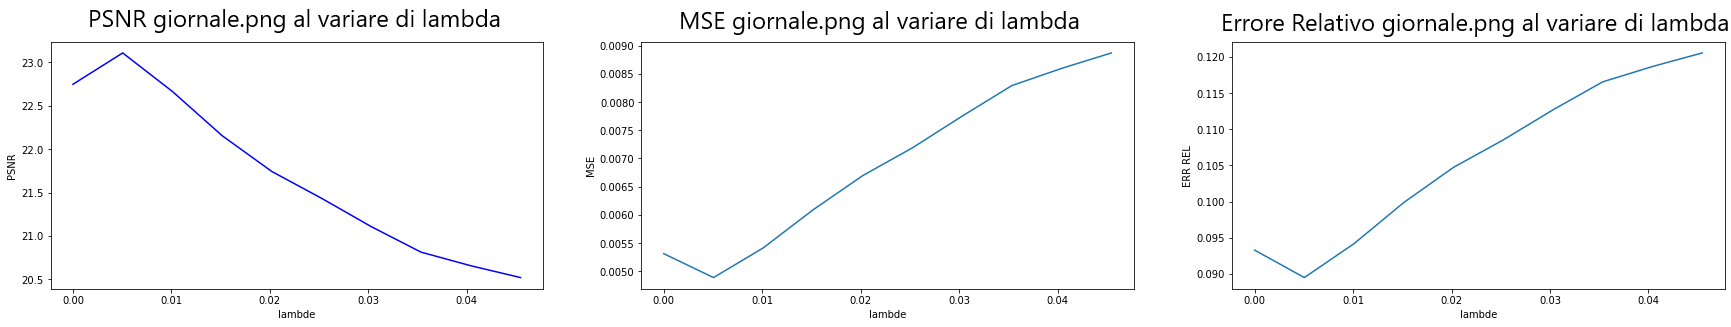
\includegraphics[width=\textwidth]{imgRel/graficoGiornale.png}
    
\includegraphics[width=\textwidth]{imgRicostruzione/ricostruzioneGiornale_TOTVAR_maxPSNR23.20.png}
    \caption{Immagine Originale, Immagine Corrotta, Immagine Ricostruita e i relativi grafici di variazione PSNR, MSE ed Errore Relativo (da sinistra a destra)}
\end{figure}